%\section{Introduction}
\section{Background} 
Driving assistance is becoming crucial in the modern era for covering long distances by road, but achieving semi-autonomous driving functionality comes with caveats as it has not reached the level of safety humans expect from a modern machine. The goal of this paper is to make a leap forward in making semi-autonomous driving a safer feature through synthetically generating adverse road conditions and training it to bridge the safety gap in autonomous driving. Achieving human-level driving capabilities requires bridging this gap in simulated driving datasets. Currently, collecting real-world data to train driving models is prohibitively expensive and logistically dangerous. The cost of physically recreating "edge cases" such as multi-car pileups or pedestrians darting out in heavy fog is a burden that ultimately falls on the end-user. Synthetic data generation via computer simulation offers a revolutionary solution to this problem [2]. Unlike real-world collections, synthetic generation provides researchers with high-level control over generation metrics.
 \\


\section{Rational of the Study}

This paper aims to achieve full safe driving on the road. Modern Autonomous Vehicles has reached self-driving capabilities as we expect, but with earlier versions of it having flaws along with. This is due to reasons varying from overwhelming the onboard computers with sensory data to corner cases of unpredictable human behavior. Car crash investigations gave us quite a lot of knowledge on how the model works while driving on road. Car accidents take away thousands of life every year. Autonomous vehicle crashes occur due to reasons such as different car sensors(LiDAR, Radar) oscillating between multiple object classification and responses to different objects, leading to discarded tracking, then to reasons like reaction lag, where the system takes a short time to compute and prevent false positives at the moment of impact. Even reasons such as humans engaging auto-drive mode, giving less attention to driving, and at the moment of a sudden collision they take time to gain consciousness of the moment. Although autonomous vehicles suffer mostly from classification errors, Waymo, a car driving technology company, as mostly solved this issue with their NIEON (Non-Impaired, Eyes always ON) human model and their L4 model, which persistently tracks and classifies objects, allowing them to outperform even idealized human models through which Waymo reduced crash injuries to about 92\%. This paper aims to generally improve the accuracy even further. \\
This paper also aims to bridge the existing gap in the simulated driving dataset to reach the driving capabilities achieved by humans. This can be done through computer generated sumulations, a core necessity in achieving driving safety. The problem with driving on the road and collecting data to train driving models is that it is usually very expensive in nature, and this cost has to be beared by the end user. So, solving this issue can be revolutionary to automated driving assistance, which can be achieved by generating data, synthetically, through computer image generation \cite{Leudet2018Virtual}. Synthetically generated datasets will allow researchers to have a high-level control over the generation metrics, such as driving scenarios in heavy fog, heavy rain, clogged up vision sensors, complex traffic scenes, driving edge cases etcetera. Making a model to work perfectly requires a large portion of a training dataset, and synthetic data generation just happens to be the perfect choice for medium cost with high effectiveness. \\
Training data volume aside, diversity in training data and quality of data are also crucial in training a model. Problems such as overfitting, which is a neural network learning all training data but losing the ability to generalize, which in concept is a failure of the Bias-Variance trade-off can make model predictions unreliable. Model entropy is the capability of a network models parameter distribution with extremely high randomness or noise, a crucial concept in information theory and statistical learning, refering to the variety of functions a model can fit, which in concept is a deep neural network (DNN) with millions of parameters, that represents a hypothesis space with massive complexity (often discussed in terms of VC-dimension or Rademacher complexity). Problems such as exploding gradient, which is the need for specific activation functions, which in concept is during backpropagation, gradients are calculated via the chain rule, involving repeated multiplication of the weight matrices, can become unstable if a large amount of generated data is provided. To make training efficient, we considered these problems and made synthetic data generation efficient to make model training and prediction effective.

\section{Problem Statement}
The scarcity of sufficient training data, often the unavailability of general driving data, is the gap that this paper aims to reduce. Critical safety events, such as pedestrians crossing the road directly in front of the vehicle, occur most often in countries in the South Asian region, making it easy to collect data for robust model prediction training. There are no training data for 3-wheelers, a common medium of transportation in countries like Bangladesh, India, and Pakistan. Also, the on-road traffic behavior is different from the Western countries. So, generating synthetic data for training driving models, to eradicate the region specificity, will also result in significant accuracy in model performance.\\

\begin{figure}[h]
    \centering
    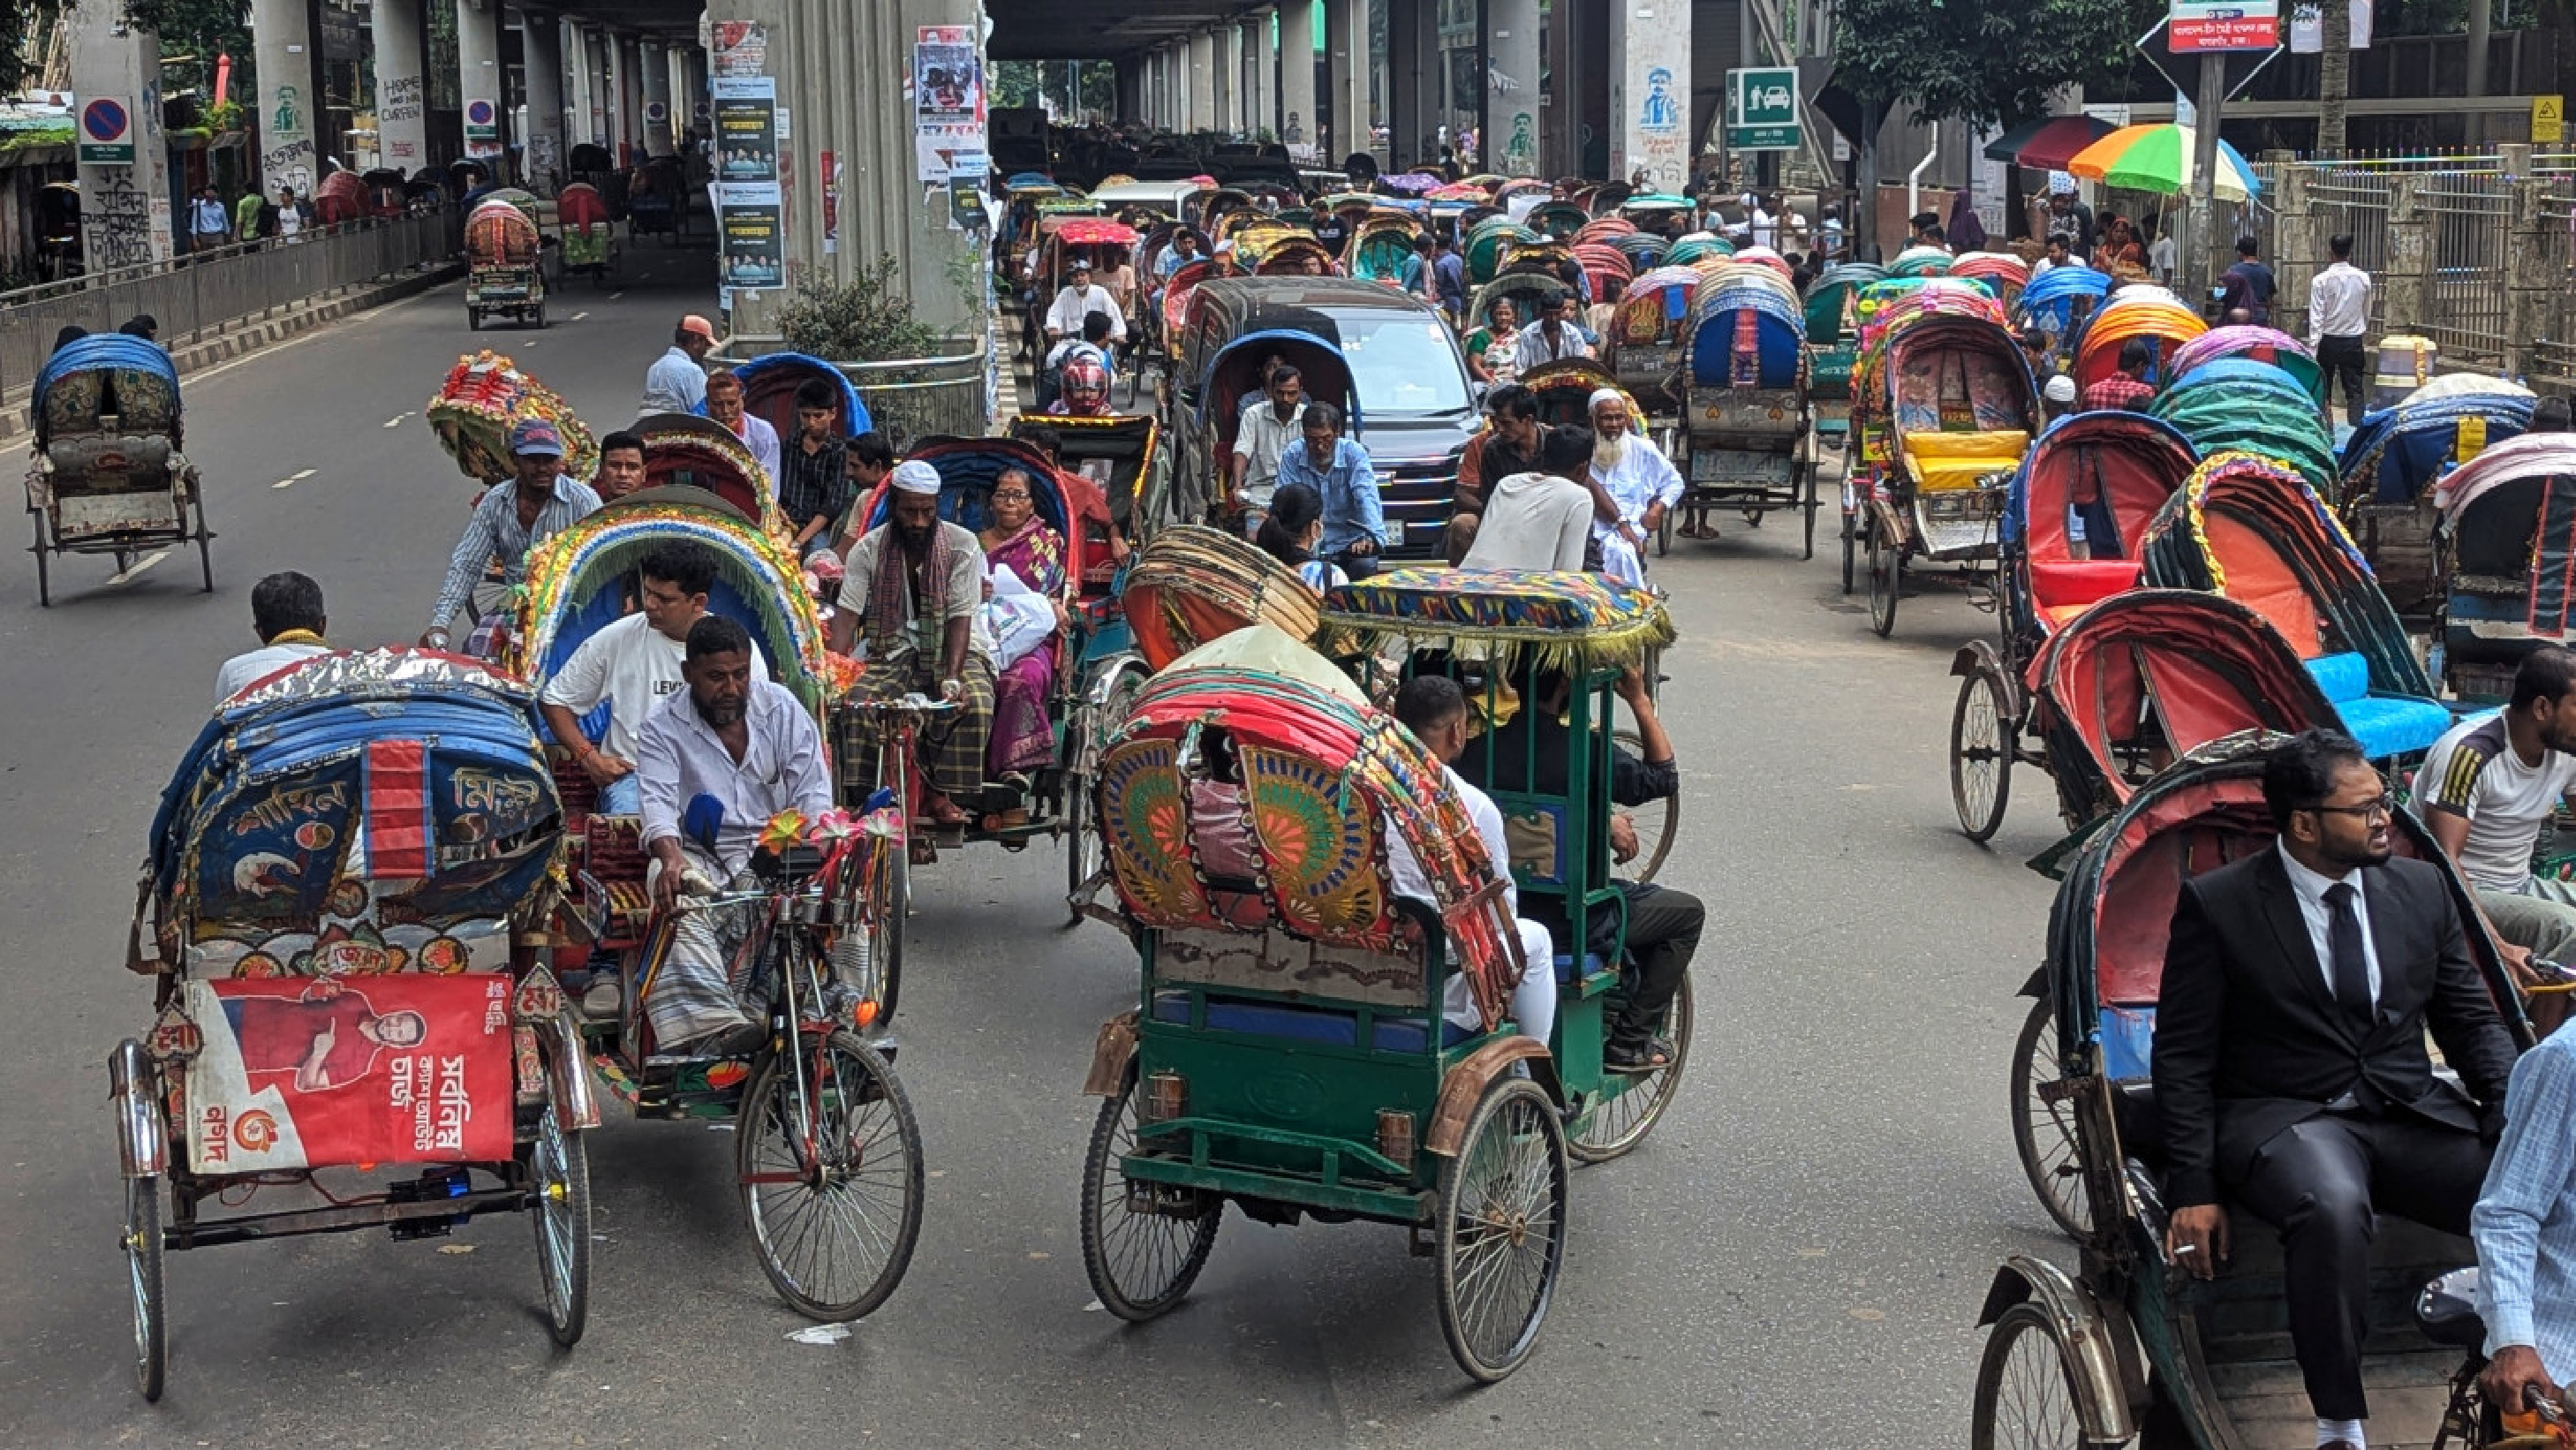
\includegraphics[width=9cm]{images/rickshaw_gathering.pdf}
    % \hyperref[]{Gathering Rickshaws, adapted from \url{https://www.tbsnews.net/features/panorama/illegal-and-unchecked-growing-menace-wrong-side-driving-dhaka-1213781#lg=\1&slide=0}.}
    \label{fig:sample}
\end{figure}
\begin{figure}[h]
    \centering
    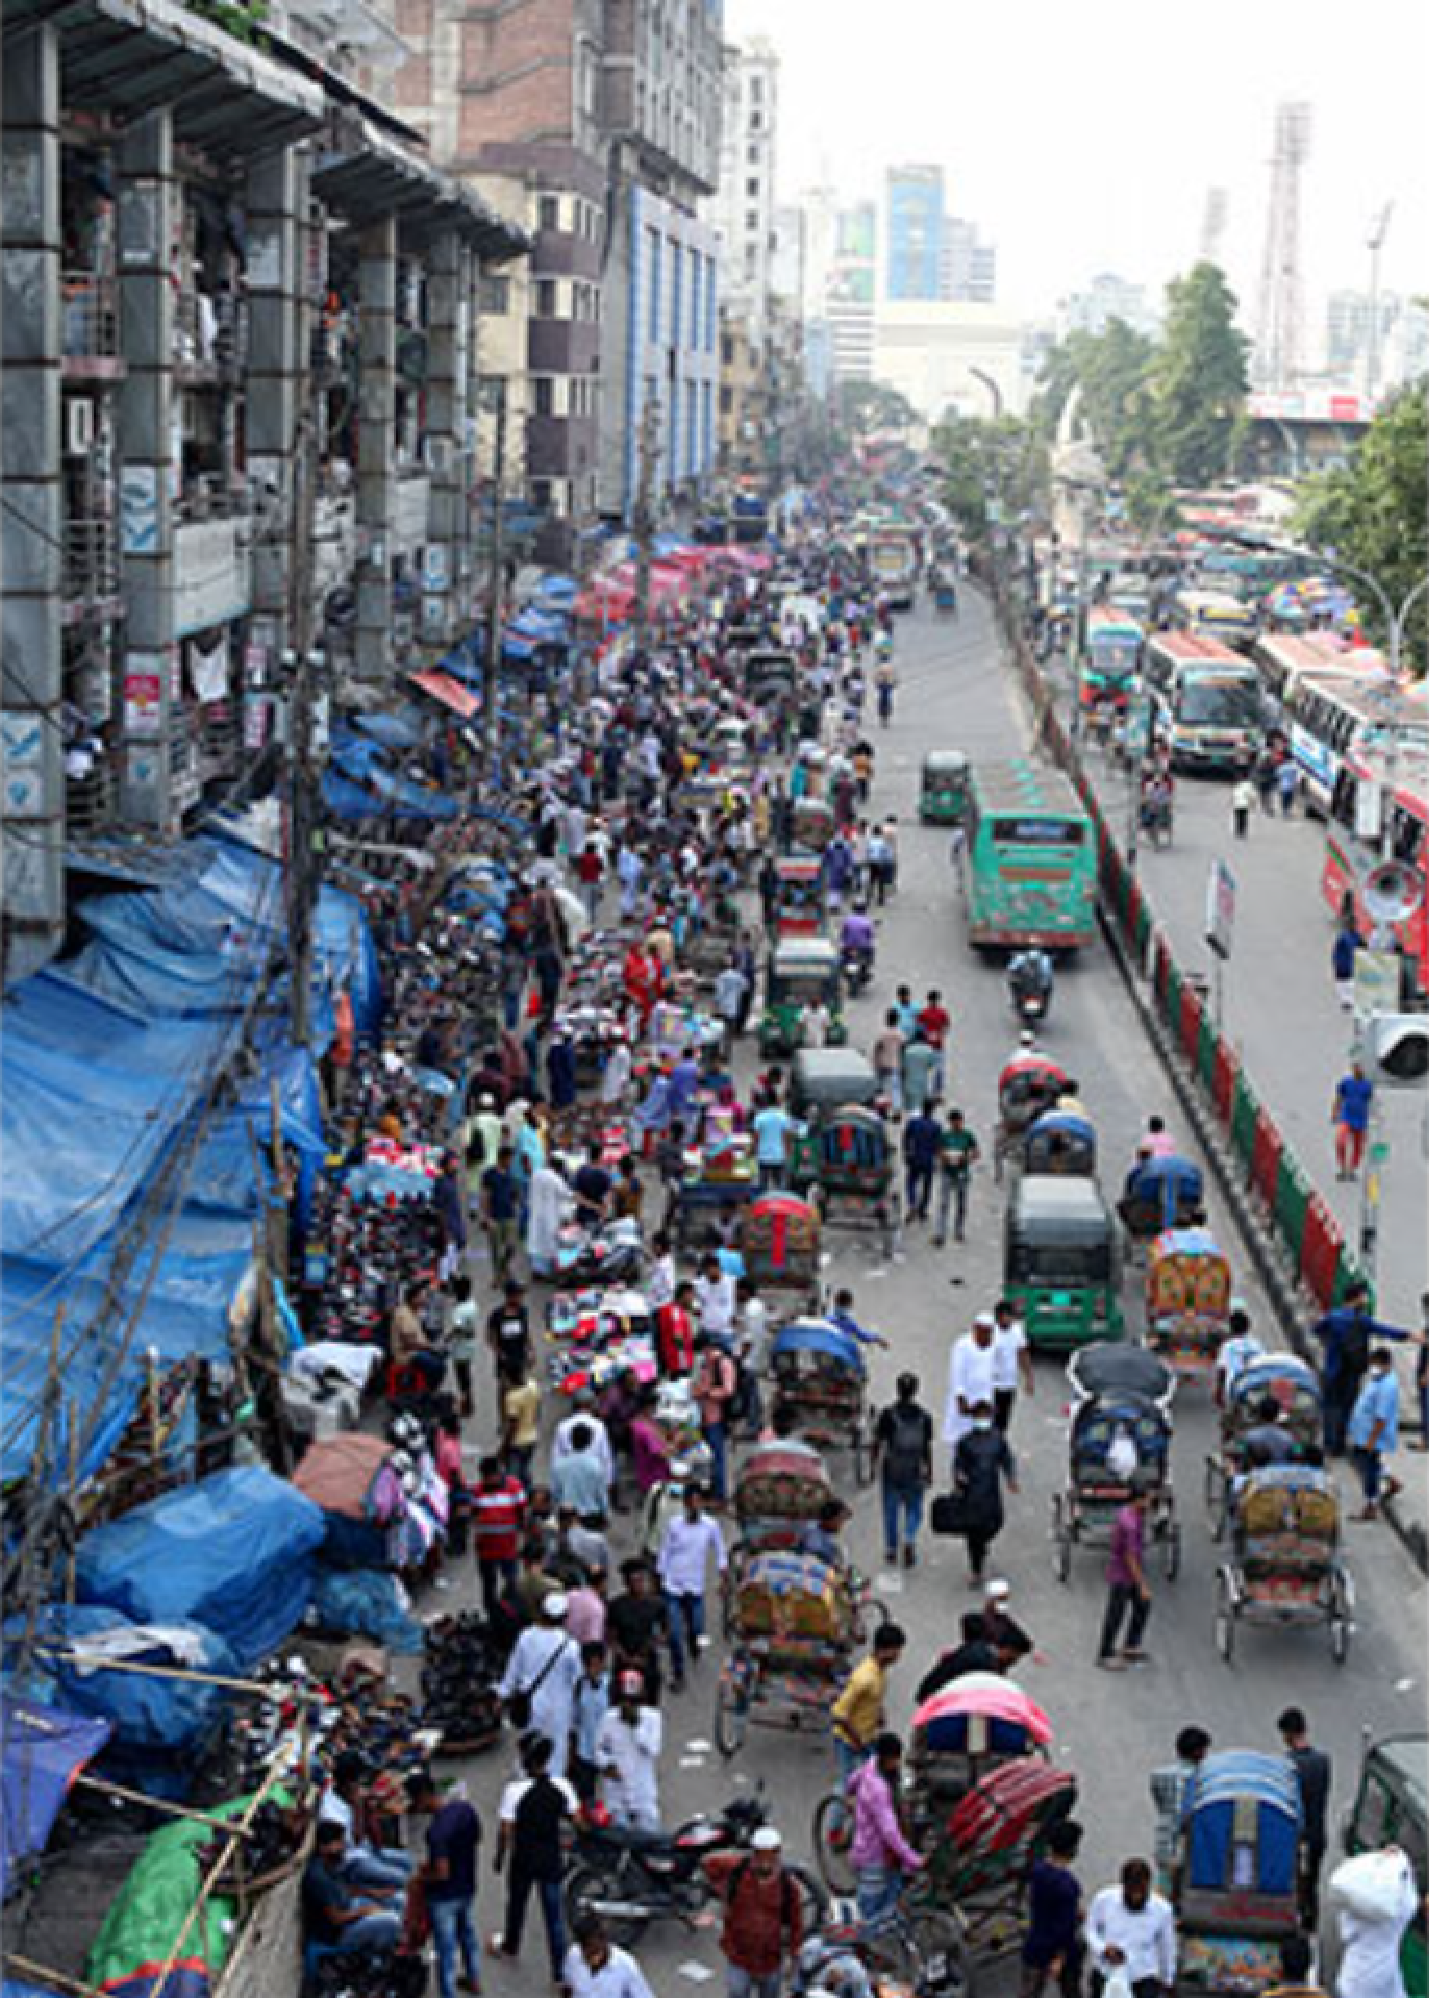
\includegraphics[width=4cm]{images/Pedestrian.pdf}
    \caption{Gathering Pedestrians, adapted from \url{https://en.bonikbarta.com/bangladesh/iuyHDYXARmGfr9lA}.}
    \label{fig:sample}
\end{figure}


\section{Objective}

The main goal of our research is to build a strong system for creating synthetic data. This system will simulate traffic conditions that are chaotic and mixed like that of South Asia. To achieve this, we must appeal to a large-scale data factory that can produce scenes on the fly that can look like scenes from the roads of Bangladesh without endangering any camera crew. Today's roads are autonomous, and they reflect that. That is the starting point, and our study attempts to take a step to address the issue.

We have three concrete objectives in our mind as we study: 
\\

\textbf{Indigenous Asset Creation:}They will not reliably detect one on the road if they had never seen a Nosimon or an easy-bike in training. To solve this, we create realistic visualizations of these vehicles, which are not part of nuScenes, BDD100K or any other public benchmark available today.\\

\textbf{Adverse Scenario Simulation:} Complex driving scenarios with non-lane following of cars will be simulated. The scenarios will be based on the “Drivership” of the local driving community. Variations in vehicles entering and out, and the "creeping" of traffic will be modeled. Unpredictable pedestrian behaviour will also be incorporated such as jaywalking in busy urban environments.\\

\textbf{Pretraining \& Validation:} : We want to show that it helps to pretrain models for object detection. We will use YOLO architectures for this test. First, we will train them using our synthetic data set. We will then evaluate them using actual video footage of roads in South Asia. Hopefully this will help them to more easily identify and classify local vehicles.\\

\section{Methodology in Brief } 
The methodology constructs a synthetic data factory with real dashcam data and enriches it with images from AI image editing creating rare, dangerous and dangerous scenarios that would not otherwise be possible or feasible to film intentionally. Each generated frame is first created based on a real road photo-graph (including its true geometry, lighting and infrastructure), and then Stable Diffusion XL is tasked with painting an agent or event into a precisely outlined area of the image, using three structural maps generated from the original scene and a text prompt that describes exactly what is supposed to appear, and how surrounding traffic should react. Some vehicle classes, such as rickshaws or auto-rickshaws, that are rarely encountered by the base model are also served by a small number of targeted adapters, trained on just a handful of images per class, yielding agents that are truly local instead of merely approximated. When we need to show the motion, not just one moment, our pipeline will create 2 endpoint frames and give them to a separate video model, which will fill in the motion in between, creating physically believable motions instead of blending pixels. The output may be a single photo or a video clip, and it goes through an automatic verification step to ensure the photo contained the objects the detector was looking for, to accurately boundary the objects' pixel footprint, to ensure that if the objects were in a physical scene, it followed basic physical laws, and to directly write the resulting bounding boxes to the same annotation format that is used for training the detector, without any manual labelling. The final dataset combines these synthetic and real-world data sets: the detector is first trained on the synthetic data to learn the rare concepts and then fine-tuned on real footage, and whenever the pipeline's output is below quality thresholds, the settings are adjusted and the entire generation run again until the output reaches the required quality.
\begin{figure}[h]
    \centering
    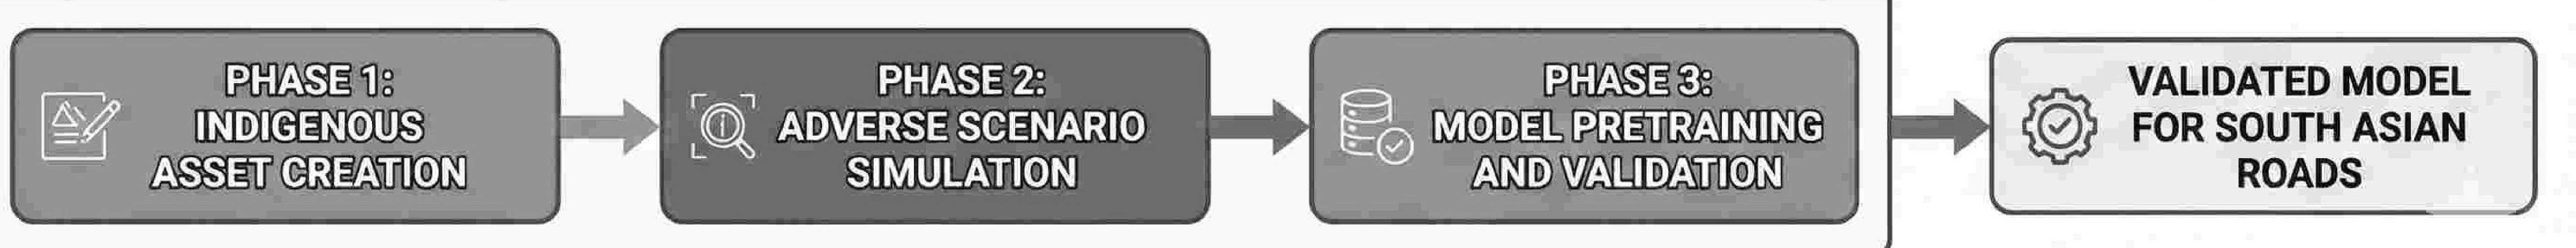
\includegraphics[width=9cm]{images/flowchart.pdf}\\
    \caption{Research Methodology}
    \label{fig:methodology}
\end{figure}

\section{Scopes and Challenges}
The scope of our work is deliberately narrow not because the broader problem is uninteresting, but because doing one thing well matters more than doing everything partially. What we are specifically trying to close is the gap between what standard datasets contain and what South Asian roads actually look like. That focus shapes everything below.\\

\textbf{Region-Specific Asset Generation:} The most immediate gap is visual. Standard datasets like nuScenes, BDD100K, and their peers simply do not contain auto-rickshaws, battery-powered easy-bikes, or the range of three-wheelers that make up a substantial fraction of Bangladeshi road traffic. Creating accurate visual representations of these vehicles is the foundation everything else rests on.\\

\textbf{Unstructured Scenario Simulation:} We limit our research to urban, mixed-traffic environments. These areas are known for non-lane-based driving. We focus on generating specific difficult scenarios. Examples include pedestrians walking on the road, sudden cut-ins by small vehicles, and driving through intersections without traffic lights.\\

\textbf{Perception Task Focus:} TPath planning and full end-to-end driving are deliberately out of scope here. What we are testing is narrower: whether a vision-based detector specifically a YOLO model which does becomes meaningfully more accurate at recognising local vehicle classes after being exposed to our synthetic data. That is the one question we are set up to answer.\\

\textbf{Pretraining Methodology:} Our experimental claim is that pretraining on region-specific synthetic data gives the model a head start that carries through into the fine-tuning stage. Because BadODD is small, a model arriving at it with no prior exposure to local classes will struggle to generalise from it. We want to find out how much of that struggle disappears when the synthetic pretraining phase is included.\\

However, our study faces several technical and logistical limits:\\

\textbf{The Reality Gap:} The sim-to-real problem is not something we have fully solved even no one has. Even with diffusion-based generation starting from real photographs, there will be artifacts and texture inconsistencies that do not appear in genuine dashcam footage. Whether those imperfections are enough to limit what the detector actually learns from the synthetic data is something we will have to measure rather than assume.\\

\textbf{Behavioral Fidelity:} For us, arguably the harder limitation is behavioral. South Asian traffic runs on a kind of ongoing negotiation between road users subtle gestures, reading gaps, anticipating what the rickshaw three vehicles ahead is about to do — and none of our template-based scenario generation truly captures that. We can model specific events, but the underlying social logic of the street is much harder to encode.\\

\textbf{2D Asset Scarcity:} High-quality 2D models for local vehicles are not sold in stores. You cannot buy a model of a damaged "Leguna" or a "Nosimon". We must create these assets from scratch. This takes a lot of manual work. Also, our models might lack the variety of shapes found in the real world.\\

\textbf{Validation Data Scarcity:} We need real-world data to verify our results. However, annotated datasets from Bangladesh are scarce. We only have small sets like BadODD. This limits our ability to test our results on a large scale.\\


\section{Team Overview}

Our team of absolutely excellent people are conducting the research on this paper. We split our work in the same manner so that there is no gap left in our study. Rafiul Islam Rafi worked on crash statistics to find real gaps in safe driving. Anirban Roy collected thesis papers and organized them based on categories, along with reviewing papers. Mir Ryan Mahmud Shafin reviewed papers and contributed in literature review. Murchona Anika Swapnil contributed in reviewing papers.\\

\section{Key Learnings and Insights}

Based on the procurement of paper reviews, the key learning is that standard Western autonomous driving datasets are fundamentally ill-suited for the chaotic, heterogeneous traffic of South Asia due to a critical "Reality Gap" in both visual assets and behavioral logic. A major insight is the necessity of shifting from lane-based path planning to area-based navigation, as traffic in these regions operates on drivership, social, and empirical expectations rather than strict legal norms. Consequently, ourr study demonstrates that synthetic data generation is not only a cost-saving tool, but also an essential required for the future of training automobiles for driving assistance  to safely model rare, edge cases and indigenous vehicle classes (like Desi Nosimons and Rickshaws) that are absent from global datasets yet vital for local deployment.

